\documentclass[a4paper,11pt]{article}
\usepackage{graphicx}
\usepackage{caption}
\usepackage{subcaption}
\usepackage{amsmath,amssymb}
\usepackage{geometry}
\geometry{margin=25mm}
\usepackage{datetime}
\usepackage{luatexja}
\usepackage{float}
\title{Allen-Cahn方程式における界面運動の数値解析}
\author{藤原 大地(武田研 M2)}
\date{2025年6月13日}

\begin{document}

\maketitle

\section{はじめに}
Allen-Cahn方程式は二相系における界面の進展を記述する代表的な反応拡散型偏微分方程式である。
本課題では、1次元のステップ関数型初期条件および固定境界条件下において、パラメータ$a$の違いが界面の運動に与える影響を数値的に調べた。
\section{課題1}
\subsection{数値計算の条件}
使用した方程式は以下の通りである:
\[
\frac{\partial u}{\partial t} = \varepsilon^2 \frac{\partial^2 u}{\partial x^2} - (u-a)(u^2 - 1)
\]
ここで、$\varepsilon^2 = 0.5$とした。

初期条件は以下のように、ランダムな微小ノイズとした:
\[
u(x, 0) = 0.01 \times \text{randn}(x)
\]
また、境界条件は周期($u(0) = u(L)$)とした。

\subsection{結果と考察}
パラメータ$a$を $-0.5, 0, 0.5, 1.0$ に変化させて、それぞれについて時間発展を計算した。
図\ref{fig:kadai1_snapshot}には、時刻$t = 40$における$u(x,t)$の静止画像を示す。

\begin{figure}[H]
  \centering
  \begin{subfigure}[b]{0.45\textwidth}
    \centering
    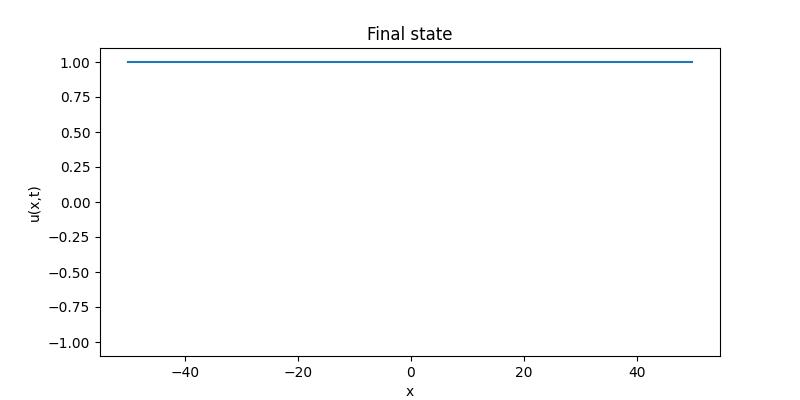
\includegraphics[width=\textwidth]{tex_gif_figures/result_am0p5_eps0p5_final.png}
    \caption{$a = -0.5$}
  \end{subfigure}
  \hfill
  \begin{subfigure}[b]{0.45\textwidth}
    \centering
    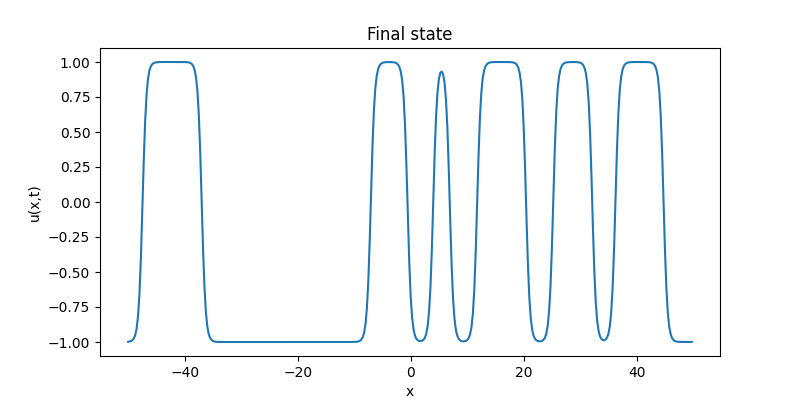
\includegraphics[width=\textwidth]{tex_gif_figures/result_a0_eps0p5_final.png}
    \caption{$a = 0$}
  \end{subfigure}

  \vspace{0.5cm}
  \begin{subfigure}[b]{0.45\textwidth}
    \centering
    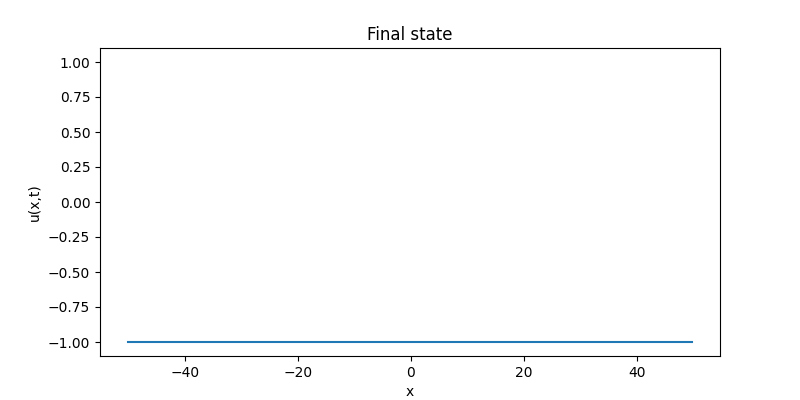
\includegraphics[width=\textwidth]{tex_gif_figures/result_a0p5_eps0p5_final.png}
    \caption{$a = 0.5$}
  \end{subfigure}
  \hfill
  \begin{subfigure}[b]{0.45\textwidth}
    \centering
    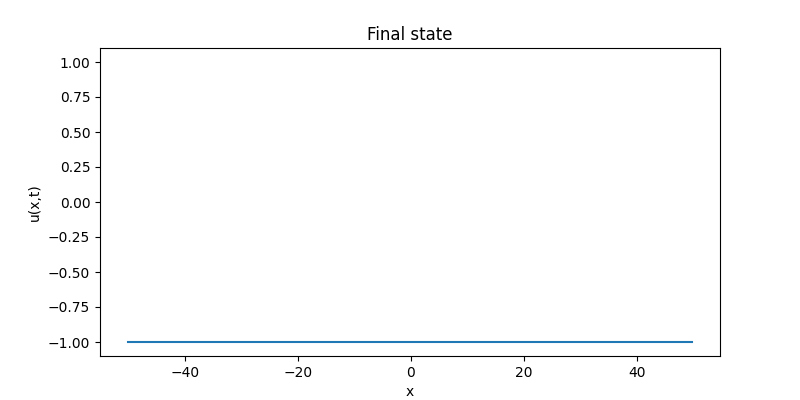
\includegraphics[width=\textwidth]{tex_gif_figures/result_a1p0_eps0p5_final.png}
    \caption{$a = 1.0$}
  \end{subfigure}
  \caption{各$a$における$u(x,t)$の時間発展($t = 40$時点、ランダム初期条件)}
  \label{fig:kadai1_snapshot}
\end{figure}

図より、初期に存在した多数のランダムな小ドメインが時間とともに粗大化し、最終的には系全体がいずれかの安定相($u = \pm 1$)へ収束する様子が確認できる。

\begin{itemize}
  \item $a = 0$:ポテンシャルが対称なため、ドメインの勝敗は初期平均により決まり、界面の縮小(粗大化)によって収束する。
  \item $a > 0$:$u = -1$側が安定なため、$+1$ドメインが押し込まれて最終的に$-1$相が支配的となる。
  \item $a < 0$:$+1$相の方が安定であり、$-1$ドメインが消滅する。
\end{itemize}

これは反応項
\[
f(u) = (u - a)(u^2 - 1)
\]
によって与えられるポテンシャル井戸の深さの非対称性に起因しており、浅い井戸の相がより安定な相に飲み込まれていくという傾向を示す。

なお、課題2で見られたような明確な界面速度は観察されにくい。これはランダム初期条件により多数の界面が存在し、それらの駆動が打ち消し合って平均的な速度が小さくなるためである。

\subsection{結論}
本課題では、周期境界条件下でランダムな初期条件を与えたAllen-Cahn方程式の数値計算を行い、ドメインの粗大化と最終状態の偏りを観察した。
ポテンシャルの非対称性により、初期のランダム分布であっても優勢な相が明確に現れることを確認した。
また、界面が互いに干渉しあうことで、課題2とは異なり明確な界面速度が得られにくい点も特徴として観察された。

\section{課題2}
\subsection{数値計算の条件}
使用した方程式は以下の通りである:
\[
\frac{\partial u}{\partial t} = \varepsilon^2 \frac{\partial^2 u}{\partial x^2} - (u-a)(u^2 - 1)
\]
ここで、$\varepsilon^2 = 0.5$とした。

初期条件は以下のステップ関数型:
\[
u(x, 0) =
\begin{cases}
-1 & (x < 0) \\
+1 & (x \geq 0)
\end{cases}
\]
また、境界条件は固定(Dirichlet)とし、$u(-L) = -1,\; u(L) = +1$と設定した。
\subsection{結果と考察}
パラメータ$a$を $-0.5, 0, 0.5, 1.0$ に変化させて、それぞれについて時間発展を計算した。
図\ref{fig:gif_evolution}には、時刻$t = 40$における$u(x,t)$の代表的な静止画像を示す。
この時点では界面の移動が顕著に現れており、各$a$における振る舞いの違いが明確に観察できる。

\begin{figure}[H]
  \centering
  \begin{subfigure}[b]{0.45\textwidth}
    \centering
    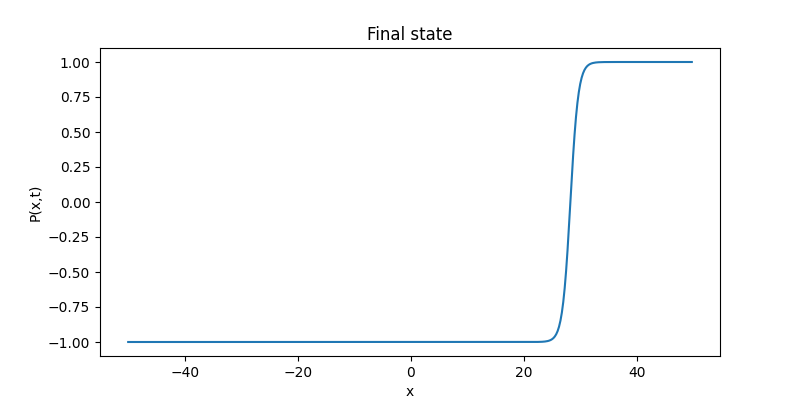
\includegraphics[width=\textwidth]{tex_gif_figures\dirichlet_a0p5_eps1_final - コピー.png}
    \caption{$a = -0.5$}
  \end{subfigure}
  \hfill
  \begin{subfigure}[b]{0.45\textwidth}
    \centering
    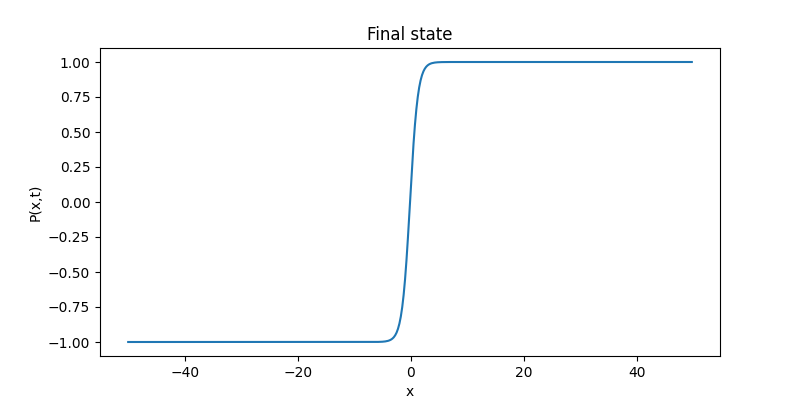
\includegraphics[width=\textwidth]{tex_gif_figures\dirichlet_a0p0_eps1_final - コピー.png}
    \caption{$a = 0$}
  \end{subfigure}

  \vspace{0.5cm}
  \begin{subfigure}[b]{0.45\textwidth}
    \centering
    \includegraphics[width=\textwidth]{tex_gif_figures\dirichlet_am0p0_eps1_final - コピー.png}
    \caption{$a = 0.5$}
  \end{subfigure}
  \hfill
  \begin{subfigure}[b]{0.45\textwidth}
    \centering
    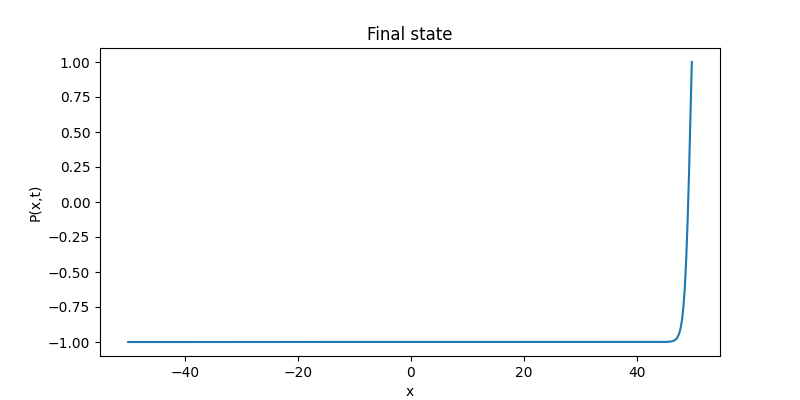
\includegraphics[width=\textwidth]{tex_gif_figures\dirichlet_a1p0_eps1_final - コピー.png}
    \caption{$a = 1.0$}
  \end{subfigure}
  \caption{各$a$における$u(x,t)$の時間発展($t = 40$時点)}
  \label{fig:gif_evolution}
\end{figure}

図より、各$a$に応じて界面の位置が大きく変化している様子が読み取れる。

\begin{itemize}
  \item $a = 0$:ポテンシャルが対称であり、$u = \pm1$は等しく安定。界面には駆動力が働かず、$t = 40$でも位置は初期のままでほぼ静止。
  \item $a > 0$:$u = -1$側の井戸が深くなるため、$-1$相がより安定に。界面は右へ移動し、$-1$相が押し広げられている。
  \item $a < 0$:$u = +1$が優勢で、界面は左に移動。$+1$相が広がる。
\end{itemize}

この挙動は、反応項
\[
f(u) = (u - a)(u^2 - 1)
\]
が与えるポテンシャル形状の非対称性によって説明できる。  
$a$の符号が井戸の深さの偏りを生み、その結果として界面が安定相へと動く。

特に $a = 0$ が \textbf{臨界値 $a^*$} に対応しており、ここで界面速度がゼロになることが理論・数値ともに一致している。
数値計算を通じて、Allen-Cahn方程式の持つ非線形性とポテンシャル構造が、界面運動を決定づけることを確認できた。
\subsection{結論}
本レポートでは、1次元Allen-Cahn方程式における界面運動を数値的に解析した。界面速度の向きはパラメータ$a$の符号に依存し、$a = 0$を臨界点として界面の移動方向が反転することを確認した。
\end{document}